\documentclass[conference]{IEEEtran}
\IEEEoverridecommandlockouts

\usepackage{cite}
\usepackage{amsmath,amssymb,amsfonts}
\usepackage{algorithmic}
\usepackage{graphicx}
\usepackage{textcomp}
\usepackage{xcolor}
\usepackage{url}
\usepackage{hyperref}
\usepackage[T1]{fontenc}
\usepackage[utf8]{inputenc}
\usepackage[ngerman]{babel}

\graphicspath{ {./images/} }

\makeatletter % changes the catcode of @ to 11
\newcommand{\linebreakand}{%
  \end{@IEEEauthorhalign}
  \hfill\mbox{}\par
  \mbox{}\hfill\begin{@IEEEauthorhalign}
}
\makeatother % changes the catcode of @ back to 12

\def\BibTeX{{\rm B\kern-.05em{\sc i\kern-.025em b}\kern-.08em
    T\kern-.1667em\lower.7ex\hbox{E}\kern-.125emX}}
\begin{document}

\title{Scradles -- Konzeptpapier
%{\footnotesize BigData, Cloud und NoSQL Sommersemester 2022}
}

\author{\IEEEauthorblockN{Asmerom Amos}
\IEEEauthorblockA{\textit{a.asmerom@oth-aw.de} \
}
\and
\IEEEauthorblockN{Boni Christoph}
\IEEEauthorblockA{\textit{c.boni@oth-aw.de} \
}
\and
\IEEEauthorblockN{Kreuzer Aaron}
\IEEEauthorblockA{\textit{a.kreuzer@oth-aw.de} \
}
\and
\IEEEauthorblockN{Rall Adrian}
\IEEEauthorblockA{\textit{a.rall@oth-aw.de} \
}
\and

\linebreakand % <----- NOTE HERE, breaking after the third one!

\IEEEauthorblockN{Tahata Djoumsi}
\IEEEauthorblockA{\textit{d.tahata@oth-aw.de} \
}
\and
\IEEEauthorblockN{Wöllmer Leonard}
\IEEEauthorblockA{\textit{l.woellmer@oth-aw.de} \
}
}

\maketitle

\begin{abstract}
    In diesem Konzeptpapier wird das Projekt "`Scradles"' von Team Gelb erläutert. Die Anwendung ist eine digitale Version des Spiels "`Schere, Stein, Papier"'.
\end{abstract}

%\begin{IEEEkeywords}
%\end{IEEEkeywords}

\section{Einleitung}
Das Projekt "`Scradles"' soll eine Web-Version des Spiels "`Schere, Stein, Papier"' werden.
Hierbei können zwei beliebige Spieler gegeneinander in einem Spiel à 3 Runden antreten.
Für die intuitive und einfache Bedienung wird ein minimalistisches Design angestrebt.

Die Anwendung soll für eine unbegrenzte Anzahl an Spielern skalierbar sein und nach optionaler Anmeldung eine Rangliste über alle Spieler führen.

\section{Verwandte Arbeiten}
"`Scradles"' soll im Layout der Desktop-Anwendung "`Schere, Stein, Papier"' von Aaron Kreuzer ähneln.
\begin{center}
    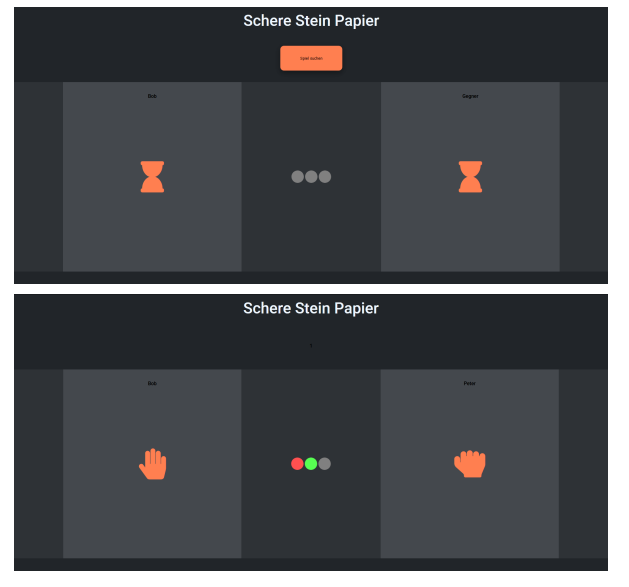
\includegraphics[width=\linewidth]{verwandt.png}
\end{center}

\section{Anforderungen - User Stories}
\subsection{Spiel starten}
\textit{Ich als} Spieler
\textit{möchte} ein Spiel durch ein Klick auf "`Spiel starten"' beginnen,
\textit{weil} ich ohne Aufwand eine schnelle Runde spielen können will.
\newline
\textbf{Akzeptanzkriterien}
\begin{itemize}
    \item Button "`Spiel Starten"' startet eine Runde gegen einen zufälligen Gegner
\end{itemize}

\subsection{Auswahl des Gegenstands}
\textit{Ich als} Spieler
\textit{möchte} mit Hilfe von drei Buttons meinen Gegenstand wählen,
\textit{weil} ich schnell und einfach meine Auswahl sehen und eine Entscheidung treffen können will.
\textbf{Akzeptanzkriterien}
\begin{itemize}
    \item Auswahl wird an den Server übertragen
    \item Auswahl wird beim Benutzer dargestellt
\end{itemize}

\subsection{Darstellung des Rundengewinners}
\textit{Ich als} Spieler
\textit{möchte} zum Rundenende visualisiert haben wer gewonnen und wer verloren hat,
\textit{weil} die Runde damit abgeschlossen wird.
\newline
\textbf{Akzeptanzkriterien}
\begin{itemize}
    \item Sobald beide Spieler eine Auswahl getroffen haben, informiert der Server die Spieler über den Gewinner der Runde
    \item Der Rundengewinner wird bei beiden Spielern dargestellt
\end{itemize}

\subsection{Timeout bei Inaktivität}
\textit{Ich als} Spieler
\textit{möchte} maximal 10 Sekunden auf die Eingabe des Gegenspielers warten müssen,
\textit{weil} das Spiel sonst zu lang dauert.
\newline
\textbf{Akzeptanzkriterien}
\begin{itemize}
    \item Während auf den Gegenspieler gewartet wird, wird dem Benutzer ein Ladesymbol datgestellt
    \item Server sendet Timeout und beendet die Runde nach 10 Sekunden ohne Eingabe
\end{itemize}

\subsection{Revanche anfordern}
\textit{Ich als} Spieler
\textit{möchte} nach dem Spiel eine Revanche anfordern,
\textit{weil} ich gegen den selben Spieler noch einmal spielen möchte.
\newline
\textbf{Akzeptanzkriterien}
\begin{itemize}
    \item Button "`Revanche"' startet neues Spiel mit den gleichen Spielern
\end{itemize}

\subsection{Darstellung des Spielgewinners}
\textit{Ich als} Spieler
\textit{möchte} am Ende des Spiels den Gewinner sehen,
\textit{weil} das Spiel damit abgeschlossen wird.
\newline
\textbf{Akzeptanzkriterien}
\begin{itemize}
    \item Sobald ein Spieler mehr als 2 Runden gewonnen hat, informiert der Server die Spieler über den Gewinner des Spiels
    \item Der Spielgewinner wird bei beiden Spielern dargestellt
\end{itemize}

\subsection{Anmeldung und Rangliste}
\textit{Ich als} Spieler
\textit{möchte} mich registrieren um Statistiken zu speichern und an der Rangliste teilzunehmen,
\textit{weil} ich mich mit anderen Spieler vergleichen möchte.
\newline
\textbf{Akzeptanzkriterien}
\begin{itemize}
    \item Die Anmeldung ist optional
    \item Die Anmeldung erfolgt über Benutzername und Passwort
    \item Der Server speichert automatisch Punkte für gewonnene Spiele
\end{itemize}

\subsection{Spiel gegen einen Freund}
\textit{Ich als} Spieler
\textit{möchte} einen bestimmten Spieler zu einer Runde einladen,
\textit{weil} ich gegen Freunde spielen können möchte.
\newline
\textbf{Akzeptanzkriterien}
\begin{itemize}
    \item Die Spieler müssen nicht angemeldet sein, um gegeneinander zu spielen
\end{itemize}

\section{Methoden}
Anfrage oder bidirektional?


Hauptfokus der Anwendung ist die \textit{containerisierte} Entwicklung um einfache Skalierbarkeit in der \textit{Cloud} zu gewährleisten. Durch Load-Balancing soll es möglich sein die Benutzeranfragen auf eine beliebige Anzahl an Servern zu verteilen. 

Für die Datenspeicherung wird eine \textit{NoSQL-Datenbank} verwendet werden.

\end{document}